\documentclass[12pt]{article}
\usepackage{amsmath}
\usepackage[T1]{fontenc}
\usepackage{graphicx}

\title{MDL 21.10}
\author{Dominik Szczepaniak}
\begin{document}

\maketitle
Zrobione:
\begin{tabular}{|| c c c c c c c c c c c||}
    \hline
    1D & 2 & 3 & 4 & 5 & 6 & 7D & 8 & 9 & 11 & 12 \\
    \hline
    N & Y & Y & Y & Y & N & Y & Y & Y & Y & Y
\end{tabular}

%TODO: 1,6,8,9
\bgroup\obeylines

\section{Zadanie 2}
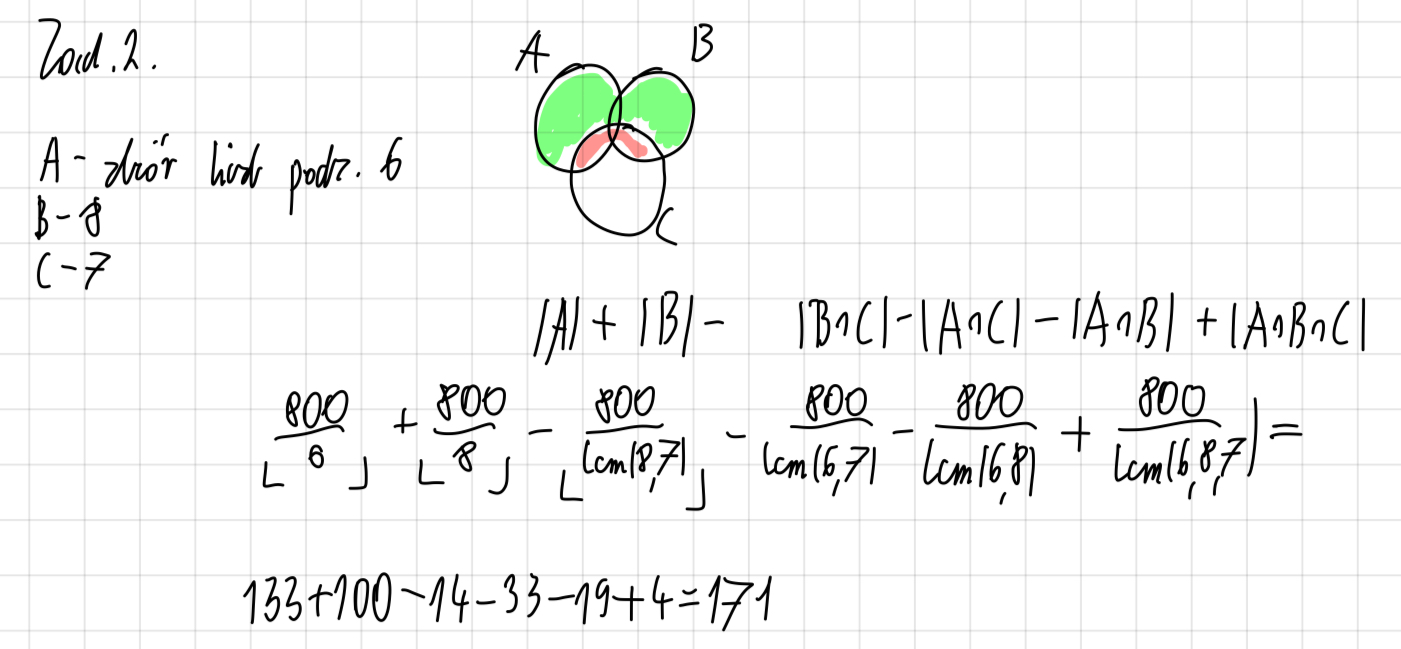
\includegraphics[width=120mm]{zad2}

\section{Zadanie 3}
Łącznie - wszystkieA - wszystkieB - wszystkieC - wszystkieAiB - wszystkie BiC - wszystkie AiC + wszystkie AiBiC
Łączna liczba opcji: 
$\frac{9!}{4!*3!*2!}$
wszystkieA (9-4+1)
$\frac{6!}{3!*2!}$
wszystkieB (9-3+1)
$\frac{7!}{4!*2!}$
wszystkieC (9-2+1)
$\frac{8!}{4!*3!}$
wszystkieAiB (9-4-3+2)
$\frac{4!}{2!}$
wszystkieBiC (9-3-2+2)
$\frac{6!}{4!}$
wszystkieAiC (9-4-2+2)
$\frac{5!}{3!}$
wszystkieAiBiC (9-4-3-2+3)
$\frac{3!}{3!}$ 

$\frac{9!}{4!*3!*2!} - \frac{6!}{3!*2!} - \frac{7!}{4!*2!} - \frac{8!}{4!*3!} - \frac{4!}{2!} - \frac{6!}{4!} - \frac{5!}{3!} + \frac{3!}{3!} = 754$


\section{Zadanie 4}
Baltazar Gąbka ma 7 przyjaciół. Określ na ile sposobów może zapraszać po 3 z nich na kolację przez 7 kolejnych dni tak, aby każdy z nich został zaproszony przynajmniej raz.

Zapraszać 7 przyjaciół każdego dnia może na P($\binom{7}{3}$, 7) sposobów. 
Jeśli chcemy omijać jednego przyjaciela, to mamy $\binom{7}{1}$ opcji na wybranie przyjaciela i $P(\binom{6}{3}, 7)$ wyboru spośród reszty, więc łącznie $\binom{7}{1} * P(\binom{6}{3}, 7)$.
Dwóch przyjaciół możemy omijać na $\binom{7}{2} * P(\binom{5}{3}, 7)$ sposobów.
Trzech przyjaciół możemy omijać na $\binom{4}{3} = 4$ możliwe grupy 3 osobowe, a potrzebujemy przynajmniej 7 (jedna na każdą noc), więc to możemy pominąć i dalsze kroki też
Łączny wynik wynosi więc:
$P(\binom{7}{3}, 7) - \binom{7}{1} * P(\binom{6}{3}, 7) + \binom{7}{2} * P(\binom{5}{3}, 7)$ =
$\frac{35!}{28!} - 7*\frac{20!}{13!} + 21! * \frac{10!}{3!}$ = 
$51090942202866115200$

\section{Zadanie 5}
Udowodnijmy, że $\sum_{k=0}^n \binom{n}{k}^2$ równa się liczbie dróg, po których wieża może przejść z lewego dolnego rogu do prawego górnego rogu szachownicy $(n+1) \times (n+1)$ poruszając się wyłącznie do góry lub na prawo.

Krok na pole (i, j) można zrobić z (i-1, j) lub (i, j-1). Czyli albo idąc w góre albo w prawo. Ten proces zajmuje więc 2n kroków, gdzie n kroków to kroki w górę, a n kroków to kroki w prawo. Zatem liczba dróg to $\binom{2n}{n}$. I tyle równa się zwinięta suma. 

Obliczmy teraz ilość dróg do górnego pola licząc najpierw drogi z (0, 0) do (k, n-k) a później z (k, n-k) do (n, n). Zauważmy, że każda z tych dróg ma długość n. k $\in {1, 2, 3, ..., n}$ 
Zauważmy, że ilość dróg do (k, n-k) jest równa $\binom{n}{k}$, bo możemy wybrać dowolną ilość kroków k w dowolną stronę. Droga z (k, n-k) do (n, n) będzie liczyć n-k kroków w prawo i k kroków w góre. Czyli liczba możliwych dróg jest równa $\binom{n}{n-k}=\binom{n}{k}$.

Także całkowita liczba kroków z (0,0) do (n,n) która przechodzi przez (k, n-k) jest równa iloczynowi możliwych dróg z (0,0) do (k, n-k) i dróg z (k, n-k) do (n,n). Także jest równa $\binom{n}{k} * \binom{n}{k} = \binom{n}{k}^2$.
Sumowanie po wszystkich możliwych k $\in {1, 2, 3, ..., n}$ daje nam łączną liczbę dróg, czyli:
$\sum_{k=0}^{n} [\binom{n}{k}^2]$ co jest równe $\binom{2n}{n}$

\section{Zadanie 6}

Trzy punkty mogą być pokolorowane dwoma kolorami na 8 sposobów, więc jeśli wybierzemy 9 linii to muszą być dwie linie pokolorwane w ten sam sposób. Połączmy te linie pionową kreską i mamy prostokąt. 
ZZZ
ZZC
ZCZ 
ZCC 
CZZ
CZC 
CCZ 
CCC
\section{Zadanie 7}
Wybieramy n+1 liczb spośród kolejnych 2n liczb naturalnych.
Zauważmy, że każda liczba jest zapisana jako albo $2^k$ * liczba nieparzysta. Liczby nieparzyste są ze zbioru {1,3,5,...,2n-1}. Więc co najwyżej możemy wziąc n takich wartości. 
Teraz włóżmy nasze n+1 liczb do odpowiednich szufladek która mówi o największym nieparzystym dzielniku. Zauważmy, że jeśli wzięliśmy n+1 liczb to musi istnieć szufladka, która ma co najmniej 2 elementy.
Wejdźmy więc do tej szufladki. Obie te liczby są postaci $2^k * l$, gdzie l to ta największa liczba nieparzysta, która dzieli tą liczbę.
Pierwszą liczbą niech będzie $2^k * l$, a drugą $2^m * l$ i niech k>m (równie nie mogą być, bo każda liczba ma być różna).
Oznaczmy te liczby jako a i b.
Więc 
a = $2^k * l$, 
b = $2^m * l$ 
$\frac{a}{b} = \frac{2^k * l}{2^m * l}$ => $a = 2^{k-m} * b$
Także b dzieli a. 

\section{Zadanie 8}
Mamy przypadek ze stars and bars. Możemy zapisać przedmioty jako gwiazdki i rozdzielic do 10 miejsc.
Mamy więc 50+9 przedmiotów i 9 miejsc do rozdzielenia, odpowiedzią jest więc
$\binom{59}{9}$

Ogólny wzór dla n przedmiotów i k szuflad (rozróżnialnych) to:
$\binom{n+k-1}{k-1}$



\section{Zadanie 9}


wszystkich opcji: $\binom{100+4-1}{4-1}$

x1+x2+x3+x4=100
x1, x2 <= 29
x3, x4 <= 39

$Wynik = N - N_{x1>29} - N_{x2>29} - N_{x3>39} - N_{x4>39} - N_{x1>29 and x2>29} - N_{x1>29 and x3>39} - N_{x1>29 and x4>39} - N_{x2>29 and x3>39} - N_{x2>29 and x4>39} - N_{x3>39 and x4>39} - N_{x1>29 and x2>29 and x3>39} - N_{x1 > 29 and x2>29 and x4>39} - N_{x1 > 29 and x3>39 and x4>39} - N_{x2 > 29 and x3>39 and x4>39} + N_{x1>29 and x2>29 and x3>39 and x4>39}$

$N = \binom{103}{3}$
$N_{x1>29} = \binom{73}{3}$
$N_{x2>29} = \binom{73}{3}$
$N_{x3>39} = \binom{63}{3}$
$N_{x4>39} = \binom{63}{3}$
$N_{x1>29 and x2>29} = \binom{43}{3}$
$N_{x1>29 and x3>39} = \binom{33}{3}$
$N_{x1>29 and x4>39} = \binom{33}{3}$
$N_{x2>29 and x3>39} = \binom{33}{3}$
$N_{x2>29 and x4>39} = \binom{33}{3}$
$N_{x3>39 and x4>39} = \binom{23}{3}$
$N_{x1>29 and x2>29 and x3>39} = \binom{4}{3}$
$N_{x1 > 29 and x2>29 and x4>39} = \binom{4}{3}$
$N_{x1 > 29 and x3>39 and x4>39} = 0$
$N_{x2 > 29 and x3>39 and x4>39} = 0$
$N_{x1>29 and x2>29 and x3>39 and x4>39} = 0$

Więc razem mamy:
$\binom{103}{3} - 2*\binom{74}{3} - 2*\binom{64}{3} - 4*\binom{35}{3} - \binom{25}{3} - \binom{45}{3} - 2*\binom{16}{3} - 2*\binom{6}{3} = 140, 400$

\section{Zadanie 10}

$10^6 \equiv 1 (mod 7)$
$10^{100000 mod 6} = 10^4$
$10^4 \equiv 4 (mod 7)$
$10^{100000} - 4 dzieli sie na 7$

\section{Zadanie 11}
Liczba naturalna a, której zapis w systemie dziesiętnym to $a_{n}a_{n-1}...a_2a_1a_0$ dzieli się przez 11 wtw gdy liczba $\sum_{i=1}^{\lceil{\frac{n}{2}}\rceil} a_{2i-1} - \sum_{i=1}^{\lfloor{\frac{n}{2}}\rfloor} a_{2i}$ dzieli się przez 11.

Jest to prawdziwe stwierdzenie. Mamy, że 
$\sum_{i=1}^{\lceil{\frac{n}{2}}\rceil} a_{2i-1} - \sum_{i=1}^{\lfloor{\frac{n}{2}}\rfloor} a_{2i}$ $\equiv 0 (mod 11)$
co jest równoważne
$\sum_{i=1}^{\lceil{\frac{n}{2}}\rceil} a_{2i-1} (mod 11) \equiv \sum_{i=1}^{\lfloor{\frac{n}{2}}\rfloor} a_{2i} (mod 11)$ 

Weźmy dowolną liczbę naturalną k. Możemy ją zapisać jako 
$k = \sum_{i=0}^{l} a_i * 10^i$ gdzie $a_i \in {0, 1, 2, 3, 4, 5, 6, 7, 8, 9}$ oraz l jest największą liczbą naturalną, która spełnia $10^l \leq k$.
Zauważmy, że $10 \equiv -1 (mod 11)$
Więc 
$k = 10^l*a_l + 10^{l-1}*a_{l-1} + ... + 10^1*a_1 + 10^0*a_0$ $\equiv$ $(-1)^l*a_l + (-1)^{l-1}*a_{l-1} + ... + (-1)^1*a_1 + (-1)^0*a_0$ $\equiv$ $\sum_{i=0}^{l} (-1)^i*a_i (mod 11)$ 
Jeśli więc rozdzielimy tą sumę na liczby parzyste i nieparzyste mamy:
$\sum_{i=0}^{l} (-1)^i*a_i (mod 11)$ $\equiv$ $\sum_{i=0}^{\lfloor{\frac{l}{2}}\rfloor} a_{2i} - \sum_{i=0}^{\lceil{\frac{l}{2}}\rceil} a_{2i+1} (mod 11)$
Także aby powyższa suma się dzieliła to musi być równa 0 modulo 11, czyli 
$\sum_{i=0}^{\lfloor{\frac{l}{2}}\rfloor} a_{2i} (mod 11)$ $\equiv$ $\sum_{i=0}^{\lceil{\frac{l}{2}}\rceil} a_{2i+1} (mod 11)$
A to jest to co chcieliśmy pokazać.

\section{Zadanie 12}

Liczbe $74^{74}$ mozemy zapisac jako $74^{64+8+2}$ 
$74 \equiv 71 mod 100$
$74^2 \equiv 76 mod 100$
$74^4 \equiv 76*76 mod 100 \equiv 76 mod 100$
$74^8 \equiv 76*76 mod 100 \equiv 76 mod 100$
...
$74^{64} \equiv 76 mod 100$

$74^{64+8+2} \equiv 76*76*76 mod 100 \equiv 76 mod 100$


\egroup
\end{document}